\chapter{TECHNICAL SPECIFICATIONS AND ARCHITECTURE}

\section{System Requirements and Specifications}
The CivicTwin system is designed to execute as a high-performance, distributed cyber-physical platform supporting concurrent spatial queries, real-time hydrodynamic evaluations, and responsive GIS map rendering. The operational hardware and software specifications are detailed in Table~\ref{tab:system_specs}.

\begin{table}[h!]
\centering
\caption{System Hardware and Software Specifications}
\label{tab:system_specs}
\fontsize{9pt}{11pt}\selectfont
\begin{tabular}{|p{3.5cm}|p{5.5cm}|p{4.5cm}|}
\hline
\textbf{Subsystem} & \textbf{Component / Tool} & \textbf{Version / Configuration} \\
\hline
\textbf{Client Platform} & Modern Web Browser & Google Chrome 120+, Mozilla Firefox 120+ \\
\textbf{Frontend Framework} & React.js with Vite Build Engine & React 18.2, Vite 5.0, JavaScript (ES2022) \\
\textbf{Geospatial Visualization} & Leaflet GIS with React-Leaflet & Leaflet 1.9.4, React-Leaflet 4.2.1 \\
\textbf{UI Styling \& Icons} & Custom Responsive CSS \& Lucide Icons & Vanilla CSS3, Lucide-React \\
\hline
\textbf{Analytics Engine} & Python Runtime Environment & Python 3.11.9 (64-bit) \\
\textbf{REST API Framework} & FastAPI with Uvicorn ASGI Server & FastAPI 0.109+, Uvicorn 0.27+ \\
\textbf{Numerical Processing} & NumPy, Pandas, NetworkX & NumPy 2.4.6, Pandas 3.0.5, NetworkX 3.6.1 \\
\textbf{Machine Learning} & Scikit-Learn Framework & Scikit-Learn 1.4+ (RandomForestClassifier) \\
\hline
\textbf{Backend Gateway} & Node.js Runtime & Node.js 18.x / 20.x LTS, Express.js 4.18 \\
\textbf{Spatial Database} & PostgreSQL with PostGIS Spatial Extension & PostgreSQL 15+, PostGIS 3.3+ \\
\textbf{Database Driver} & Node-Postgres Connection Pool & pg 8.11+, dotenv \\
\hline
\textbf{Development OS} & Operating System Platform & Microsoft Windows 11 / Linux Ubuntu 22.04 LTS \\
\textbf{Hardware Specifications} & Processor \& Memory & Intel Core i7 / AMD Ryzen 7, 16 GB DDR4 RAM \\
\hline
\end{tabular}
\end{table}

\section{High-Level System Architecture}
CivicTwin follows a modular, three-tier cyber-physical architecture designed for real-time responsiveness and data integrity. Figure~\ref{fig:sys_arch} illustrates the architectural blocks, communication interfaces, and data pipelines connecting the physical municipality to the virtual operations twin.

\begin{figure}[h!]
\centering
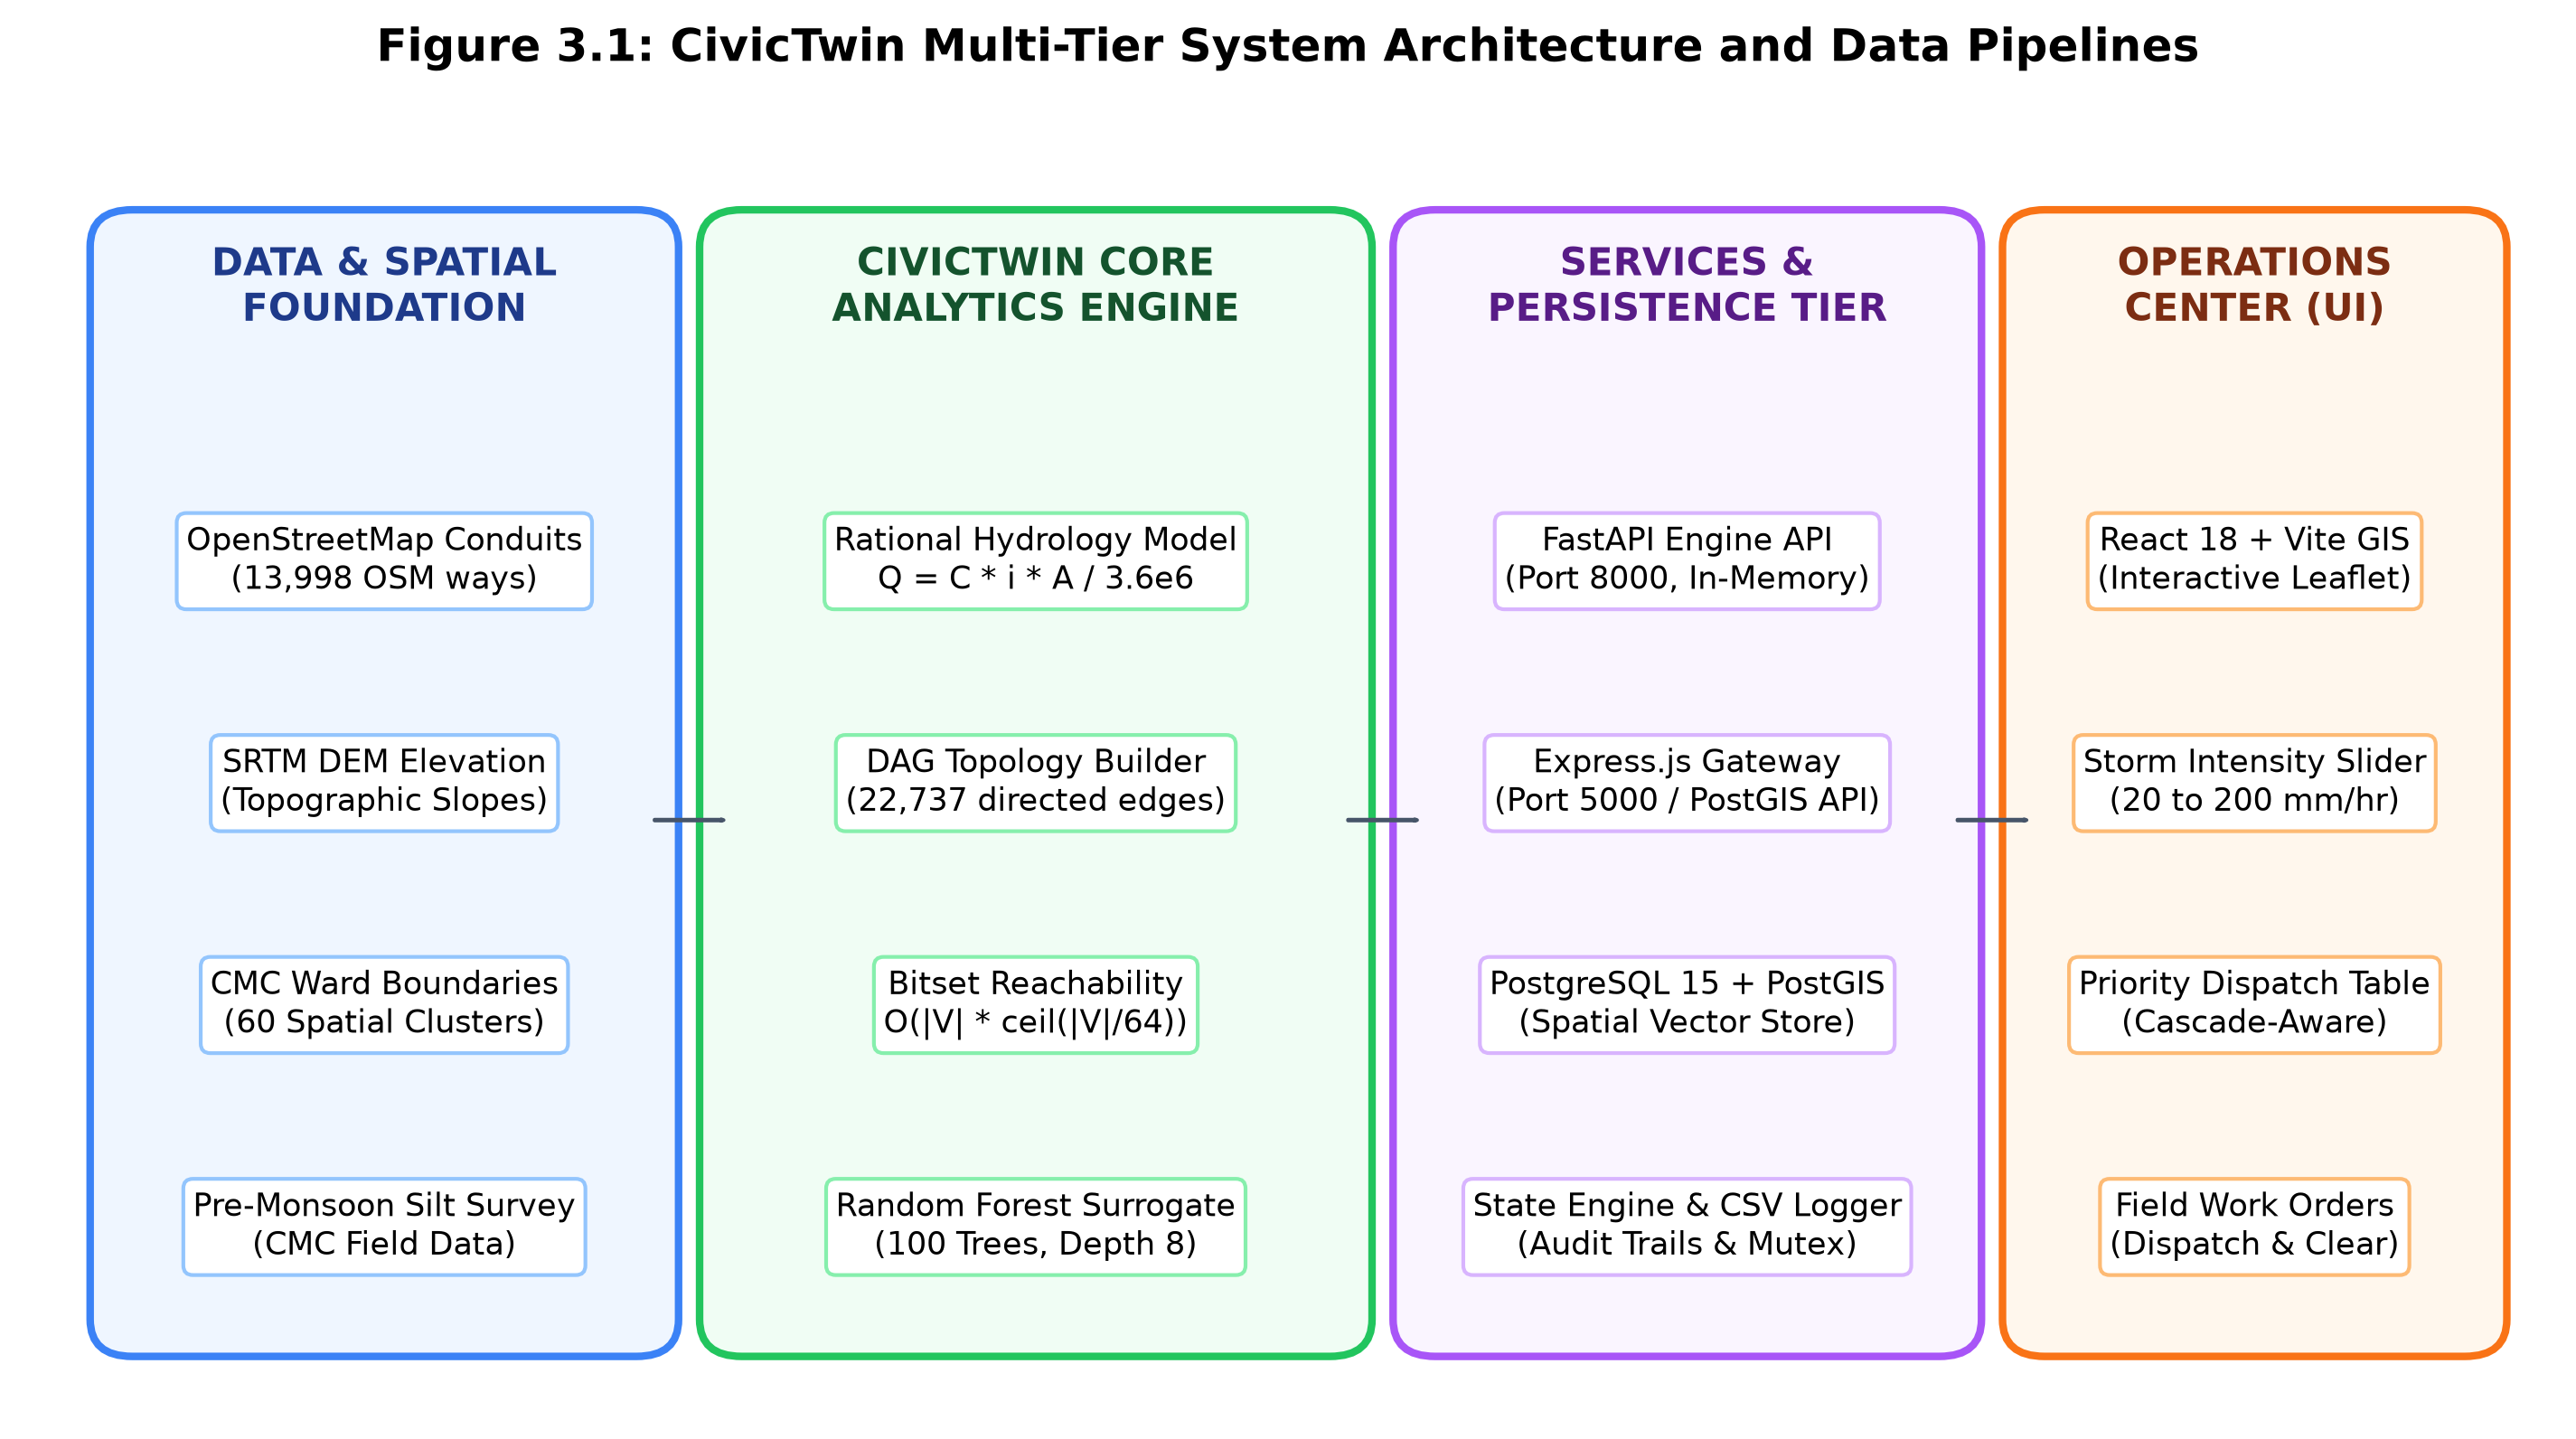
\includegraphics[width=0.98\textwidth]{figures/fig_system_architecture.png}
\caption{CivicTwin Multi-Tier System Architecture and Data Pipelines}
\label{fig:sys_arch}
\end{figure}

The architecture comprises four core operational layers:
\begin{enumerate}
    \item \textbf{Data Ingestion and Spatial Foundation:} Aggregates vector conduit geometries from OpenStreetMap (OSM) via Overpass API/OSMnx \cite{boeing2017osmnx}, digital elevation model (DEM) rasters from the NASA Shuttle Radar Topography Mission (SRTM) at 30-meter resolution, official Vellore Municipal Corporation (CMC) ward boundary polygons, and field sediment survey logs.
    \item \textbf{Core Analytics Engine (Python / FastAPI):} Maintains the in-memory Directed Acyclic Graph (DAG) of the 13,998 conduit segments. It executes the rational runoff model, computes hydraulic capacity utilisation ratios under dynamic precipitation scenarios, evaluates topological reachability via bitsets, and runs the Random Forest surrogate classifier.
    \item \textbf{Services and Persistence Tier (Express / PostGIS):} Manages transactional persistent storage of spatial conduit features in a PostgreSQL/PostGIS database. It provides an Express.js API gateway at port 5000 for spatial vector insertions, alongside an atomic JSON state file and CSV dispatch history audit log managed by the Python engine at port 8000.
    \item \textbf{Operations Command Center (React / Vite):} Provides an interactive geospatial dashboard at port 5173. Municipal engineers can manipulate storm rainfall intensity sliders (20--200~mm/hr), filter across 60 administrative zones, inspect priority dispatch queues, issue work orders to field crews, and export audit trails.
\end{enumerate}

\section{Spatial Data Modeling and PostGIS Database Schema}
To support geospatial storage, topological routing, and spatial joins with ward boundaries, CivicTwin implements a relational spatial schema within PostgreSQL utilizing the PostGIS extension \cite{obe2021postgis}. Conduits are stored as multi-segment LineStrings in geographic coordinates (EPSG:4326 - WGS84). 

The primary relational table, \texttt{drain\_conduits}, is structured as follows:
\begin{lstlisting}[language=SQL, caption={PostGIS DDL Schema for Drainage Conduits}, label={lst:postgis_schema}]
CREATE EXTENSION IF NOT EXISTS postgis;

CREATE TABLE drain_conduits (
    drain_id VARCHAR(64) PRIMARY KEY,
    ward_number INTEGER NOT NULL,
    drain_type VARCHAR(32) DEFAULT 'Open Concrete',
    width_m NUMERIC(5, 2) DEFAULT 1.50,
    depth_m NUMERIC(5, 2) DEFAULT 1.20,
    elevation_m NUMERIC(6, 2) NOT NULL,
    slope_pct NUMERIC(5, 2) DEFAULT 0.50,
    design_capacity_m3s NUMERIC(6, 3) NOT NULL,
    blockage_ratio NUMERIC(4, 3) DEFAULT 0.00,
    start_node_id BIGINT,
    end_node_id BIGINT,
    geom GEOMETRY(LineString, 4326) NOT NULL
);

-- Spatial GiST index for fast bounding-box viewport queries
CREATE INDEX idx_drain_conduits_geom ON drain_conduits USING GIST (geom);
\end{lstlisting}

Spatial indexing via GiST (Generalized Search Tree) allows the system to execute sub-millisecond bounding box filtering, enabling the client viewport culling algorithm to render only the conduit segments currently visible within the operator's browser window.

\section{RESTful API Architecture and Integration}
The system exposes two complementary RESTful API services:
\begin{enumerate}
    \item \textbf{Python Analytical Engine Endpoints (FastAPI, Port 8000):} Designed for in-memory, zero-latency analytical operations.
    \begin{itemize}
        \item \texttt{GET /api/py/top?k=\{k\}\&rain=\{rain\}\&ward=\{ward\}\&strategy=\{strat\}}: Returns the top-$k$ ranked conduits requiring desilting, active in-progress queues, real-time KPI aggregates, and total network exposure.
        \item \texttt{POST /api/py/dispatch}: Transitions a conduit from \texttt{OPEN} to \texttt{IN\_PROGRESS}, assigning it to a field desilting crew and recording pre-dispatch metrics.
        \item \texttt{POST /api/py/cleaned}: Marks an \texttt{IN\_PROGRESS} conduit as \texttt{CLEARED}, resetting its silt accumulation to 5.0\%, recalculating upstream exposure relief, and logging metrics.
        \item \texttt{POST /api/py/silt}: Permits municipal inspectors to update surveyed silt percentages for open drains following ground verification.
        \item \texttt{GET /api/py/history}: Exports the complete dispatch and clearing history log as a structured CSV document.
        \item \texttt{POST /api/py/reset}: Resets the simulation engine state to initial survey baselines for testing.
    \end{itemize}
    \item \textbf{Node.js Spatial Gateway Endpoints (Express, Port 5000):} Designed for transactional database storage and survey data ingestion.
    \begin{itemize}
        \item \texttt{GET /api/drains/spatial}: Retrieves all conduit records formatted as standard GeoJSON feature collections via PostGIS \texttt{ST\_AsGeoJSON}.
        \item \texttt{POST /api/drains/spatial}: Inserts new field-surveyed drain lines constructed from GPS coordinate pairs using \texttt{ST\_MakeLine}.
    \end{itemize}
\end{enumerate}

\section{Concurrency Control and Audit Trail Logging}
Because multiple municipal supervisors or dispatch operators may interact with the digital twin concurrently, state integrity is maintained through multi-tiered concurrency controls:
\begin{itemize}
    \item \textbf{Reentrant Thread Synchronization:} All state mutations (dispatching conduits, recording clearing completions, or resetting parameters) within the Python engine are protected by an internal reentrant mutex lock (\texttt{threading.RLock()}), preventing race conditions during simultaneous API calls.
    \item \textbf{Atomic State Persistence:} The active engine state is written to a temporary JSON file (\texttt{engine\_state.json.tmp}) before replacing the primary state file via atomic operating system replacement (\texttt{os.replace}), guaranteeing resilience against process crashes or power disruptions.
    \item \textbf{Immutable Audit Trail:} Every operational action (\texttt{DISPATCH\_ASSIGNED}, \texttt{CLEANING\_COMPLETED}, or \texttt{SURVEY\_UPDATE}) is appended to an append-only CSV audit file (\texttt{civictwin\_dispatch\_history.csv}) capturing timestamps, segment IDs, pre/post silt levels, pre/post threat levels, cascade relief metrics, storm rainfall intensity, and instantaneous network risk exposure before and after the action.
\end{itemize}
